\documentclass{beamer}
\usepackage{geometry}
\usepackage[english]{babel}
\usepackage[utf8]{inputenc}
\usepackage{amsmath}
\usepackage{amsfonts}
\usepackage{amssymb}
\usepackage{tikz}
\usepackage{graphicx}
\usepackage{venndiagram}

%\usepackage{pgfplots}
%\pgfplotsset{width=10cm,compat=1.9}
%\usepackage{pgfplotstable}

\setlength{\headheight}{26pt}%doesn't seem to fix warning

\usepackage{fancyhdr}
\pagestyle{fancy}
\fancyhf{}

%\rhead{\small{21 May 2018}}
\lhead{\small{BECA / Dr. Huson / 12.1 IB Math}}

%\vspace{1cm}

\renewcommand{\headrulewidth}{0pt}


\title{12.1 IB Math - Unit 5: Integration}
\subtitle{Bronx Early College Academy}
\author{Christopher J. Huson PhD}
\date{4 January 2019}

\begin{document}

\frame{\titlepage}

\section[Outline]{}
\frame{\tableofcontents}

\section{5.1 Drui: Antiderivatives. Friday 4 January}
\frame
{
  \frametitle{GQ: How do we find the antiderivative of a function?}
  \framesubtitle{CCSS: F.IF.B.6 Calculate \& interpret the rate of change of a function \hspace{\stretch{1}} \alert{5.1 Friday 4 January}}

  \begin{block}{Do Now. Find $\frac{\mathrm{d}y}{\mathrm{d}x}$}
  \begin{enumerate}
      \item Given $y=x^3+x^2+17$.
      \item Given $y=\frac{1}{4}x^4+\frac{1}{2}x^2+9-\frac{1}{x}$.
      \item If $\displaystyle \frac{\mathrm{d}y}{\mathrm{d}x}=3x^2+x$, find $y$.
      \item Skills check \#1 p. 290
  \end{enumerate}
  \end{block}
  Problem sets from January 2,3; Sigma notation, p 290 \\*[5pt]
  Lesson: Antiderivatives pp. 291-2\\*[5pt]
  Exam review \\*[5pt]
  Homework: Exercises 9A p. 293; test corrections due Monday
}

\section{5.2 Drui: Indefinite Integral. Monday 7 January}
\frame
{
  \frametitle{GQ: How do we find the indefinite integral of a function?}
  \framesubtitle{CCSS: F.IF.B.6 Calculate \& interpret the rate of change of a function \hspace{\stretch{1}} \alert{5.2 Monday 7 January}}

  \begin{block}{Do Now. Find the antiderivative, $F(x)$, of each function, $f(x)$, such that $F'(x)=f(x)$}
  \begin{enumerate}
      \item $f(x)=4x^3+3x^2+1$.
      \item $f(x)=x^4+x^2+5$.
      \item $f(x)= \sqrt{x}$
  \end{enumerate}
  \end{block}
  Test corrections due, review. (take home test tomorrow)\\*[5pt]
  Lesson: Indefinite integral pp. 293-4\\*[5pt]
  Homework: Exercises 9B p. 294
}

\section{5.3 Drui: Deltamath Integration Tuesday 8 January}
\frame
{
  \frametitle{GQ: How do we integrate functions?}
  \framesubtitle{CCSS: F.IF.B.6 Calculate \& interpret the rate of change of a function \hspace{\stretch{1}} \alert{5.3  Tuesday 8 January}}

  \begin{block}{Do Now. Handout-test review}
    %\begin{enumerate}

    %\end{enumerate}
  \end{block}
  Deltamath Integration practice (taking antiderivatives)\\*[5pt]
  Homework: Deltamath project through Thursday
}

\section{5.4 Drui: Boundary conditions. Wednesday 9 January}
\frame
{
  \frametitle{GQ: How do we apply boundary conditions to an integral?}
  \framesubtitle{CCSS: F.IF.B.6 Calculate \& interpret the rate of change of a function \hspace{\stretch{1}} \alert{5.4 Wednesday 9 January}}

  \begin{block}{Do Now. Find each indefinite integral.}
  \begin{enumerate}
      \item $\int (3x^2+2x+1) \,\mathrm{d}x$.
      \item $\int (x^4+6x^2+1) \,\mathrm{d}x$.
      \item $\int \sqrt{x} \,\mathrm{d}x$.
      \item $\displaystyle \int \frac{\pi}{4} \sqrt[3]{x^2} \,\mathrm{d}x$
      \item $\int x^{-1} \,\mathrm{d}x$
  \end{enumerate}
  \end{block}
  Lesson: Finding the constant $C$ given boundary conditions. pp. 295-6\\*[5pt]
  Homework: Exercises 9C p. 296-7
}

\section{5.5 Drui: Deltamath Integration Thursday 10 January}
\frame
{
  \frametitle{GQ: How do we integrate functions?}
  \framesubtitle{CCSS: F.IF.B.6 Calculate \& interpret the rate of change of a function \hspace{\stretch{1}} \alert{5.5  Thursday 10 January}}

  \begin{block}{Do Now. Handout-test review}
    %\begin{enumerate}

    %\end{enumerate}
  \end{block}
  Deltamath Integration practice (taking antiderivatives)\\*[5pt]
  Homework: Complete Deltamath calculus project
}

\section{5.6 Drui: Compositions of linear functions. Friday 11 January}
\frame
{
  \frametitle{GQ: How do we integrate compositions of linear functions?}
  \framesubtitle{CCSS: F.IF.B.6 Calculate \& interpret the rate of change of a function \hspace{\stretch{1}} \alert{5.6 Friday 11 January}}

  \begin{block}{Do Now. Derivatives and antiderivatives. (Use the chain rule)}
  \begin{enumerate}
    \item $f(x)=e^{3x}$. Find $f'(x)$.
    \item $f(x)= \ln (5x+3)$. Find $f'(x)$.
    \item $f(x)= (2x-5)^3$. Find $f'(x)$.

    \item Find $\int 4(x^2+x+1) \,\mathrm{d}x$.
    \item $y'=2x^3-1$ and $y=3$ when $x=1$. Find $y$ in terms of $x$.
    \item Given $f'(x)=\sqrt[3]{x}$ and $f(0)=1$, find $f(x)$.
  \end{enumerate}
  \end{block}
  Lesson: Antiderivatives of form $\int f(ax+b) \,\mathrm{d}x$. pp. 297-9\\*[5pt]
  Homework: Exercises 9D, 9E (odds) p. 298, 300
}

  \section{12.1 Drui}
  \frame
  {
    \frametitle{GQ: How do we calculate area with integration?}
    \framesubtitle{CCSS: F.IF.B.6 Calculate \& interpret the rate of change of a function}

    \begin{block}{Do Now}
    \begin{enumerate}
        \item Find $\int{(4x^3-3x+1)}\mathrm{d}x$.
        \item Find $\int e^{5x}\mathrm{d}x$.
        \item Find $\displaystyle \int \frac{1}{3x+1} \mathrm{d}x$.
    \end{enumerate}
    Homework review \#1, 5, 6 p. 302
    \end{block}
    Lesson: Reimann sums and the definite integral\\*[5pt]
    Task: Example 8, page 304\\*[5pt]
    Assessment: Calculator integration \\*[5pt]
    Homework: Exercises 9H evens p. 308
  }

  \section{12.1 Drui}
  \frame
  {
    \frametitle{GQ: How do we calculate area with definite integrals?}
    \framesubtitle{CCSS: F.IF.B.6 Calculate \& interpret the rate of change of a function}

    \begin{block}{Do Now}
    \begin{enumerate}
        \item Use a calculator to find $\displaystyle \int_0^{\frac{\pi}{2}}{\cos x}\ \mathrm{d}x$
        \item Differentiate $y=\sqrt{3x^3-x}$
        \item Find $\int{(6x^2-2x-5)}\mathrm{d}x$.
        \item Differentiate $y={(3x^2-5x)^5}$
        \item Find $\int 5(x^2+1)^4(2x)\mathrm{d}x$.
        \item Find $\displaystyle \int \frac{3}{x}\ \mathrm{d}x$.
    \end{enumerate}
    \end{block}
    Lesson: Properties of definite integrals p. 307\\%*[5pt]
    Task: Review homework problems\\%*[5pt]
    Assessment: Problem \#11 p. 300 \\%*[5pt]
    Homework: Exercises 9H evens p. 308
  }

  \section{12.1 Drui}
  \frame
  {
    \frametitle{GQ: How do we calculate area with definite integrals?}
    \framesubtitle{CCSS: F.IF.B.6 Calculate \& interpret the rate of change of a function}

    \begin{block}{Do Now}
    \begin{enumerate}
        \item Use a calculator to find $\displaystyle \int_{-1}^{1}{\frac{1}{x+2}}\ \mathrm{d}x$
        \item Differentiate $y=\sqrt[3]{5x^2-2x}$
        \item Find $\int{(6x^2-2)^4(12x)} \ \mathrm{d}x$.
        \item Differentiate $y={(3x^2-5x)(\ln x)}$
        \item Find $\displaystyle \int_1^2 \frac{3}{x^2}\ \mathrm{d}x$. (check your result with a calculator)
    \end{enumerate}
    \end{block}
    Lesson: The fundamental theorem of calculus p. 309\\%*[5pt]
    Task: Practice Examples 11, 12 p. 310-1\\%*[5pt]
    Assessment: Problem 9J \#1 p. 312 \\%*[5pt]
    Homework: Exercises 9I, 9J p. 310-12
  }

  \section{12.1 Drui}
  \frame
  {
    \frametitle{GQ: How do we calculate the area between two curves?}
    \framesubtitle{CCSS: F.IF.B.6 Calculate \& interpret the rate of change of a function}

    \begin{block}{Do Now: Consider the function $f(x)=-x^2+2x+3$}
    \begin{enumerate}
        \item Factor $f$ and state its zeros.
        \item Restate $f$ in vertex form. Write down the vertex as an ordered pair.
        \item Differentiate $f$. Show that the zero of $f^\prime(x)$ is the vertex of $f$.
        \item If $f(x)$ represents the height of a diver over the domain $0 \leq x \leq 3$, interpret $f(0)$ and $f^\prime(0)$
        \item What is the size of the area bounded by $f$, $x=0$, and $y=0$?
    \end{enumerate}
    \end{block}
    Lesson: The area between two functions p. 313\\%*[5pt]
    %Task: Practice Examples 11, 12 p. 310-1\\%*[5pt]
    Assessment: Example \#13 p. 314 \\%*[5pt]
    Homework: Exercises 9K p. 316
  }

  \section{12.1 Drui}
  \frame
  {
    \frametitle{GQ: How do we calculate a volume of rotation?}
    \framesubtitle{CCSS: F.IF.B.6 Calculate \& interpret the rate of change of a function}

    \begin{block}{Do Now: Sketch the functions $f(x)=10x+x^2-3x^3$ and $g(x)=x^2-2x$}
    \begin{enumerate}
        \item What are their intersections? (i.e. $f(x)=g(x)$)
        \item What is the definite integral representing the area between the curves?
        \item Using a calculator, what is the size of the area? (this may not be a trivial question)
    \end{enumerate}
    \end{block}
    Lesson: Integrating circle areas, modeling a solid p. 318\\%*[5pt]
    %Task: Practice Examples 11, 12 p. 310-1\\%*[5pt]
    Assessment: Example \#15 p. 319 \\%*[5pt]
    Homework: Exercises 9L \& 9M p. 317, 319; probability handout
  }

  \section{12.1 Drui}
  \frame
  {
    \frametitle{GQ: How do we calculate displacement from velocity?}
    \framesubtitle{CCSS: F.IF.B.6 Calculate \& interpret the rate of change of a function \qquad \alert{12.1}}

    \begin{block}{Do Now: Do the calculations below and read the handout}
    \begin{enumerate}
        \item Lance Armstrong’s average speed in his six Tour de France victories from 1999-2004 was about 24 miles per hour. Assuming that he pedals at his average speed and takes no breaks, how long would it take him to ride 38 miles to the top of a 10,000 ft. volcano?
        \item People who are not Lance Armstrong can travel at about 12 miles per hour on a bike. At that speed, how long would it take to reach the top of the volcano?
    \end{enumerate}
    \end{block}
    Lesson: Integrating velocity over time, displacement p. 321\\%*[5pt]
    %Task: Practice Examples 11, 12 p. 310-1\\%*[5pt]
    Assessment: Example \#18 p. 323 \\%*[5pt]
    Homework: Exercises 9N \& 9O p. 320, 324
  }

  \section{12.1 Drui}
  \frame
  {
    \frametitle{GQ: How do we calculate displacement from velocity?}
    \framesubtitle{CCSS: F.IF.B.6 Calculate \& interpret the rate of change of a function \qquad \alert{12.1}}

    \begin{block}{Do Now: continued, 38 mile ride in 10 hours}
    \begin{enumerate}
        \item Using the velocity vs time graph from yesterday, integrate to show that the areas representing the distance covered by the three riders are equal ($v \times t = d$).
        \item Show that a rider accelerating according to $v(t)= \frac{76}{100}t$ also arrives at $(10,38)$.
    \end{enumerate}
    \end{block}
    Lesson: Integrating velocity over time, displacement p. 321\\%*[5pt]
    Task: Review 9F, 9M, probability\\%*[5pt]
    Assessment: Example \#18 p. 323 (take home test Thursday)\\%*[5pt]
    Homework: Exercises 9P p. 326, any remaining problem sets
  }

  \section{12.1 Drui}
  \frame
  {
    \frametitle{GQ: How do we integrate a function?}
    \framesubtitle{CCSS: HSF.IF.B.6 Calculate and interpret the area under a function \qquad \alert{12.1}}

    \begin{block}{Do Now: Chain rule - Take the derivative of each function}
      \begin{enumerate}
      \item $f(x)=\sin{x^3}$
      \item $g(x)=\sqrt{x^4+2}$
      \item $h(x)=\ln{(x^2+1)}$
      \end{enumerate}
   \end{block}
    Lesson: Take home exam papers assessment \& review\\%*[5pt]
    Task: Work problems on board\\%*[5pt]
    Assessment: Test corrections due\\%*[5pt]
    Homework: Integration exam problems
  }

  \section{12.1 Drui}
  \frame
  {
    \frametitle{GQ: How do we calculate volume (of a rotated function)?}
    \framesubtitle{CCSS: HSF.IF.B.6 Calculate and interpret the area under a function \qquad \alert{12.1}}

    \begin{block}{Do Now: Identifying problem types. On your homework, underline the ``M1" points you earned. Examples:}
      \begin{enumerate}
      \item $X \sim B(10, 0.5)$
      \item bell curve sketch
      \item $u= \& \quad u'=$
      \end{enumerate}
   \end{block}
    Lesson: $\displaystyle \int_a^b \pi r^2 \text{d}x$\\%*[5pt]
    Task: Work homework problems on board\\%*[5pt]
    Assessment: self-reflection on mixed versus block problem sets\\%*[5pt]
    Homework: Solids of rotation \& mixed exam problems
  }


  \frame
  {
    \frametitle{The volume of a function rotated around the $x$-axis}
    \framesubtitle{Differentiate over $x$, but use the area of a disk defined by $A=\pi r^2$}
  \href{https://www.youtube.com/watch?v=i4L5XoUBD_Q}{video}\\
  \begin{figure}[!ht]
      \centering
      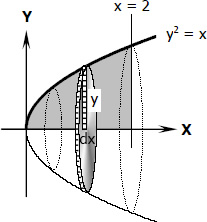
\includegraphics[width=0.5\textwidth]{0413CW-paraboloid.jpg}
  \end{figure}
  \small{Credit: MATHalino.com - Pinoy Math Community Romel Verterra}
  }

\end{document}
